Ambientes inteligentes est\~ao tornando-se realidade, este conjunto de tecnologias que est\~ao sendo desenvolvidas ser\~ao um grande passo para as \'areas como: constru\c{c}\~ao civil, industria, transporte e automa\c{c}\~ao residencial.

Para tomar decis\~oes e agirem de forma inteligente, estes ambientes necessitam de informac\c{c}\~ao sobre o contexto aonde ser\~ao implantados. As redes de sensores sem fio s\~ao um componente chave para estes ambientes, adquirem este contexto captando e  comunicando os dados do ambiente.\cite{lewis2004wireless}

Este cap\'itulo apresenta uma vis\~ao geral sobre redes de sensores sem fio, arquitetura orientada a servi\c{c}os e os protocolos de aplica\c{c}ao existentes.

\section{Redes de sensores sem fio}

Avan\c{c}os recentes nas tecnologias de sistemas eletr\^onicos, semicondutores, sensores, microcontroladores e r\'adios tornaram poss\'ivel o desenvolvimento de redes de sensores de baixo custo e baixo consumo uma realidade.

Sensores ligam o f\'isico com o mundo digital, capturando e revelando fen\^omenos do mundo real e convertendo em uma forma que pode ser processada, armazenada e utilizada para tomada de decis\~ao. A escolha entre qual sensor a ser utilizado depende muito da aplica\c{c}\~ao e da propriedade f\'sica a ser monitorada, alguns exemplos: temperatura, press\~ao, humidade, entre outros.

Um n\'o sensor de uma rede de sensores sem fio n\~ao \'e apenas respons\'avel por coletar dados, mas an\'alise da rede, correla\c{c}\~ao entre dados de outros sensores e comunica\c{c}\~ao com uma esta\c{c}\~ao base para centralizar a informa\c{c}\~ao. Isto \'e importante pois geralmente tais redes s\~ao compostas por muitos n\'os. \cite{dargie2010fundamentals}

Geralmente tais redes possuem centenas ou milhares de n\'os sensores e possuem as seguintes caracter\'isticas: pouca mem\'oria, pouco alcance do r\'adio, baixa capacidade de processamento e bateria, e custo reduzido. Comunicam-se entre si e com esta\c{c}\~oes base utilizando seus r\'adios sem f|o, permitindo dissemina\c{c}\~ao da informa\c{c}\~ao para processamento remoto, visualiza\c{c}\~ao, an\'alise e armazenamento.

Os requisitos para uma rede de sensores distribu\'ida s\~ao: reconfigura\c{c}\~ao com esta\c{c}\~ao base, controle auton\^omo de opera\c{c}\~ao e ger\^encia de energia, auto-monitoramento, efici\^encia energ\'etica para longo tempo de opera\c{c}\~ao e apta a incorporar diversos sensores.\cite{542724}

Um n\'o pertencente a esta rede geralmente \'e um dispositivo especificamente desenvolvido para um pr\'oposito, que possui poucos recursos computacionais e energ\'eticos e se comunicam entre seus semelhantes, como apresentado na figura \ref{wsnOverview}.

\begin{figure}[h]
   \label{wsnOverview}
   \centering
   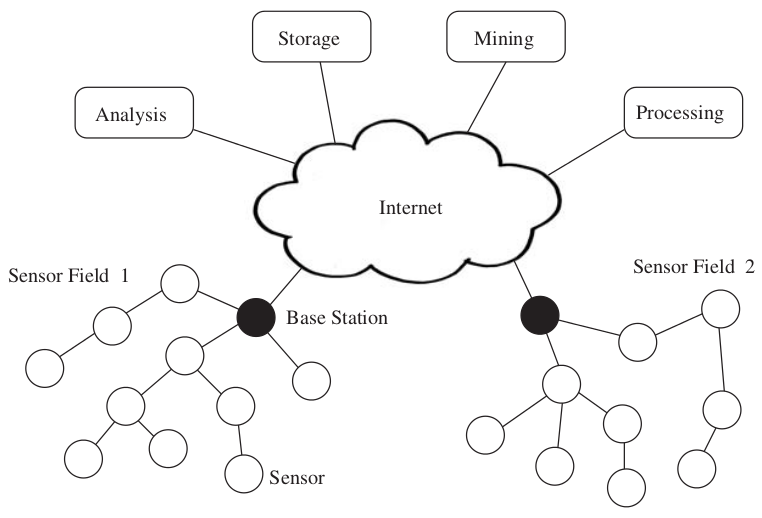
\includegraphics[width=0.7\textwidth]{figuras/wsn.png}
   \caption{Overview de uma arquitetura de redes de sensores sem fio retirado de \cite{dargie2010fundamentals}.}
\end{figure}

Muitas redes de sensores tamb\'em possuem atuadores, que permitem controle direto ao mundo real. Uma rede de sensores e atuadores recebe comandos da unidade de processamento (microcontrolador) e transforma estes comandos em sinais de entrada para um atuador, que interage com processos f\'sicos. Estas redes s\~ao chamadas de redes de sensores e atuadores sem fio, ou WSAN.

A conserva\c{c}\~ao de energia \'e um dos objetivos das redes de sensores sem fio, pois n\~ao est\~ao ligados diretamente a fonte de energia. Deve-se minimizar o consumo em todos os n\'iveis do sistema, da aplica\c{c}\~ao at\'e o meio f\'isico, iniciando com o projeto de r\'adio. \cite{WsnSurvey2008} 

\subsection{Plataforma de Hardware}

\subsection{Sistema Operacional}

\subsection{Rede de interconex\~ao}

\subsection{Aplica\c{c}\~oes}

Existe um enorme n\'umero de aplica\c{c}\~oes que pode ser desenvolvido gra\c{c}as as tecnologias de WSN.


\section{Arquitetura orientada a servi\c{c}os}

Arquitetura orientada a servi\c{c}os \'e uma forma de organizar infraestrutura e aplica\c{c}\~oes de software em um conjunto de servi\c{c}os. Estes s\~ao oferecidos por prestadores de servi\c{c}o, servidores, organiza\c{c}\~oes que implementam os servi\c{c}os, fornecem descri\c{c}\~ao dos servic\c{c}os oferecidos, suporte t\'ecnico e de neg\'ocio.

O modelo de computa\c{c}\~ao utilizando esta afirmativa \'e conhecido como Computa\c{c}\~ao Orientada a servi\c{c}os (SOC). \cite{581580}

Clientes destes servi\c{c}os podem ser outras solu\c{c}\~oes, aplica\c{c}\~oes, processos ou usu\'arios. Para satisfazer estes requis\'itos servi\c{c}os devem:
\begin{itemize}
\item Tecnologicamente neutros: utilizar-se de padr\~oes reconhecidos e bem aceitos para comunica\c{c}\~ao, descri\c{c}\~ao e mecanismos de descoberta;
\item Baixo acoplamento: detalhes desnecess\'arios (o qu\~ao desnecess\'ario precisa ser discutido) devem ser escondidos do cliente, que n\~ao precisa ter conhecimento sobre o funcionamento interno para utilizar o servi\c{c}o;
\item Localidade transparente: clientes devem ser atendidos independentemente da localidade do servi\c{c}o dispon\'ivel.
\end{itemize}

SOA n\~ao \'e apenas uma arquitetura sobre servi\c{c}os, mas um relacionamento entre tr\^es entidades: o provedor de servi\c{c} (service provider), descoberta de servi\c{c}o (service discovery agency) e o client (service requestor).  Abaixo a figura \ref{soaOverview} demonstra este relacionamento e suas intera\c{c}\~oes: publicar (publish), encontrar (find) e vincular (bind).

\begin{figure}[h]
   \label{soaOverview}
   \centering
   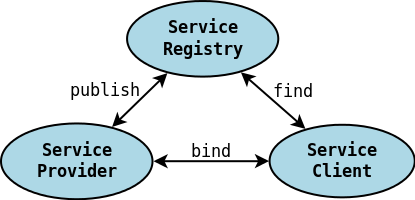
\includegraphics[width=0.6\textwidth]{figuras/soa.png}
   \caption{Arquitetura Orientada a Servi\c{c}os}
\end{figure}


\section{Webservices}

Um servi\c{c}o web \'e um sistema de software projetado para suportar interoperabilidade em intera\c{c}\~oes m\'aquina-a-m\'aquina na rede. Possui uma interface descritiva das funcionalidades num formato padronizado (especificamente WSDL). Esta nota\c{c}\~ao abstrata que deve ser implementada por um agente.\cite{w3c-web-04}. 

O agente \'e algo concreto, pode ser um peda\c{c}o de hardware ou software que recebe e envia mensagens. Um exemplo \'e implementar o mesmo servi\c{c}o web, utilizando agentes em diferentes linguagens. Embora o agente seja diferente, o servi\c{c}o Web continua o mesmo.

Servi\c{c}os Web prov\^eem um padr\~ao para a interoperabilidade entre diferentes aplica\c{c}\~oes de software, que executam em diferentes plataformas de software e hardware.


\section{Resource Oriented Architecture}

ROA \'e uma arquitetura boa para RESTful webservices. \cite{richardson2008restful}

\section{RESTful}

Uma requisic\c{c}\~ao a um webservice RESTful, utiliza a informa\c{c}\~ao do m\'etodo como um verbo HTTP e a informac\c{c}\~ao do escopo ao qual o verbo ser\'a utilizado na URI. Ao contr\'ario um estilo RPC tende a ignorar o m\'etodo HTTP, procurando pelo m\'etodo a ser utilizado e o escopo na pr\'opria URI.

Um servi\c{c}o web que utiliza HTTP e os princ\'ipios REST possui recursos e a\c{c}\~oes gen\'ericas bem definidas.\cite{rest}

Para transfe\^encia de dados utiliza-se formatos gen\'ericos que enfatizam simplicidade e usabilidade pela internet, como XML e JSON.

Os Recursos s\~ao usam um identificador \'unico e persistente, as URIs. A URIs possuem estruturas de diret\'orios, uma URI \'e uma \'arvore com ramos subordinados e superordinados conectando os n\'os. As opera\c{c}\~oes suportas s\~ao m\'etodos HTTP expl\'icitos que n\~ao salvam estado das aplica\c{c}\~oes clientes e s\~ao idempotentes, s\~ao eles:
GET: solicita ao webserver a representa\c{c}\~ao de uma informa\c{c}\~ao de um determinado recurso.
POST: criar um recurso no webserver.
PUT: mudar o estado de um recurso do webserver.
DELETE: remover o recurso ou alterar para um estado vazio.

Uma abordagem utilizando SOAP RPC em HTTP n\~ao \'e interessante para uma aplica\c{c}\~ao de RSSF, j\'a que a quantidade de informa\c{c}\~ao a ser transmitida \'e consideravelmente maior. Al\'em disso, a aplica\c{c}\~ao teria que conhecer l\'ogica interna do servi\c{c}o istrumentando o recurso utilizando chamadas de fun\c{c}\~oes remotas. A figura \ref{soaVsHttp} exemplifica e demonstra a diferen\c{c}a de uma aplica\c{c}\~ao que faz uso de SOAP RPC e outra RESTful.\cite{richardson2008restful}

%Inserir figura que demonstra a diferença entre o tamanho dos pacotes.
\begin{figure}[h]
    \label{soaVsHttp}
    \centering
    \includegraphics[width=0.7\textwidth]{figuras/soavshttp.png}
    \caption{Imagem retirada de \cite{richardson2008restful}}
\end{figure}

A figura \ref{bytesTransmitted} faz um comparativo entre o n\'umero de bytes transmitidos de diversos servidores web e seus protocolos.

\begin{figure}[h]
    \label{bytesTransmitted}
    \centering
    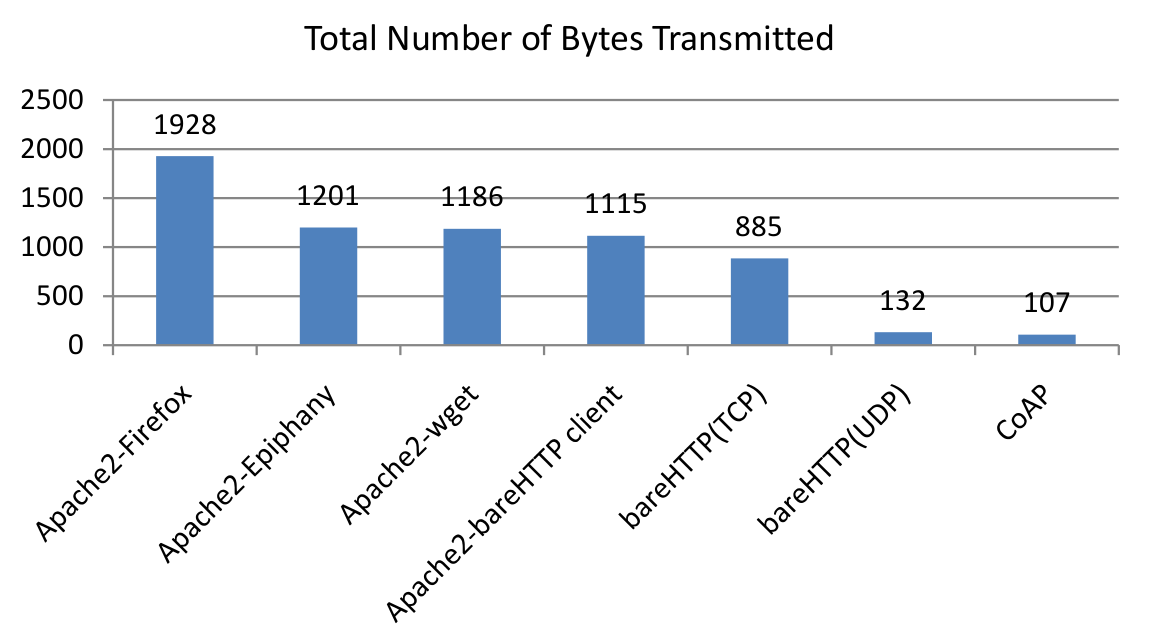
\includegraphics[width=0.7\textwidth]{figuras/bytestransmitted.png}
    \caption{Imagem retirada de \cite{transportApp}}
\end{figure}

Todos os webservices utilizam o conceito de URI, por\'em de maneiras diferentes. Mas um servi\c{c}o RESTful sempre exp\~oe a URI para cada peda\c{c}o de dado que o cliente quer operar sobre.

Os principais competidores aos servi\c{c}os web RESTful s\~ao os RPC-styles.

\section{CoAP}

Um dos principais objetivos do CoAP \'e ser uma alternativa protocolo web gen\'erico para redes com dispositivos com restri\c{c}\~ao de energia e mem\'oria.

As vantagens de utilizar um protocolo compat\'ivel com o HTTP s\~ao: a facilidade de integra\c{c}\~ao e o reuso de aplica\c{c}\~oes. CoAP \'e um conjunto REST otimizado para M2M, com suporte a descoberta de recursos, multicast e troca de mensagens ass\'incronas com simplicidade e baixo overhead.

A IETF estabelece as condi\c{c}\~oes m\'inimas para o desenvolvimento de um protocolo de aplica\c{c}\~ao compat\'ivel com HTTP, mas focado em aplica\c{c}\~oes aonde energia e mem\'oria s\~ao escassas. O protocolo CoAP foi projetado levando em considera\c{c}\~ao as restri\c{c}\~oes energ\'eticas e altas taxas de falha na transmiss\~ao dos pacotes em RSSF.

A comunica\c{c}\~ao entre os pontos no CoAP \'e de forma ass\'incrona usando o UDP. A confiabilidade \'e um par\^ametro opcional e funciona atrav\'es de um mecanismo de retransmiss\~ao exponencial. Possui 4 tipos de mensagem: Confirm\'avel, N\~ao-Confirm\'avel, Confirma\c{c}\~ao (ACK) e Reset. A figura \ref{coapFormat} mostra o formato do pacote.

\subsection{Formato das mensagens}
Uma mensagem CoAP deve caber num \'unico pacote IP, para que seja transmitida numa camada de enlace limitada.
\begin{figure}[h]
    \label{coapFormat}
    \centering
    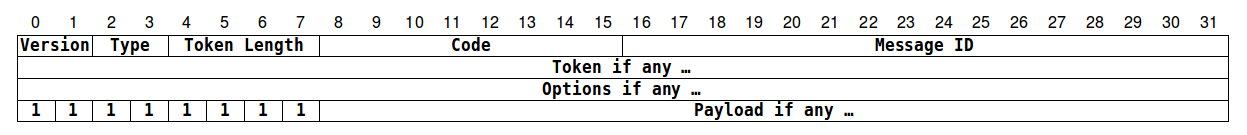
\includegraphics[width=0.6\textwidth]{figuras/formato.png}
    \caption{formato do pacote CoAP  em bits. \cite{draft-ietf-core-coap-18}}
\end{figure}


Os campos do pacote CoAP s\~ao: a vers\~ao do CoAP, implementa\c{c}\~oes devem utilizar este campo com o valor 1. O tipo: campo para definir o tipo da mensagem: Confirm\'avel (0), N\~ao-Confirm\'avel (1) , de Confirma\c{c}\~ao (2) ou Reset (3).

O tamanho do Token: utilizado para controle de requisi\c{c}\~oes e repostas. O tamanho do Token pode variar entre 0 e 8 bytes. Tamanhos entre 9 a 15 s\~ao reservados e n\~ao devem ser usados. \'E um campo sempre gerado pelo cliente CoAP.

O C\'odigo: separados em 3-bit mais significativos para classes e 5-bits menos significativos para detalhe. As classes podem indicar uma requisi\c{c}\~ao (0), uma resposta de sucesso (2), e uma resposta de erro do cliente (4), ou uma resposta de erro do servidor (5), as outras classes s\~ao reservadas. Em um caso especial o c\'odigo 0.00 indica uma mensagem vazia.

O ID da mensagem: usada para deduplica\c{c}\~ao de mensagens e confirma\c{c}\~ao ou reset de mensagens. \'E gerado por quem envia a mensagem, no caso de uma mensagem confirm\'avel ou reset, a resposta deve possuir o ID da mensagem enviada. A implemeta\c{c}\~ao da gera\c{c}\~ao dos IDs est\'a aberta, depende da aplica\c{c}\~ao que o CoAP ser\'a usado, por\'em \'e recomendado que o valor inicial seja rand\^omico.
   
%Codifica\c{c}\~ao das op\c{c}\~oes
\subsection{Transmiss\~ao de Mensagens}
A transmiss\~ao de mensagems \'e controlada basicamente pelos par\^ametros: ACK TIMEOUT, ACK RANDOM FACTOR, MAX RETRANSMIT, NSTART, Leisure e PROBING RATE.

Estes par\^ametros s\~ao respectivamente: o tempo que uma mensagem confirm\'avel aguarda o ACK; fator de randomicidade para gerar os ACK TIMEOUTs subsequentes; contador para o n\'umero m\'aximo de tentativas de retransmiss\~ao; n\'umero limite de intera\c{c}\~oes simult\^aneas mantidas por um servidor.

A Leisure \'e o tempo que o servidor aguarda para responder uma requisi\c{c}\~ao multicast, \'e calculada: $Leisure = S * G / R$. Aonde S \'e o tamanho estimado da reposta, G \'e uma estimativa do tamanho do grupo e R \'e a taxa de transmiss\~ao. PROBING RATE: \'e a taxa m\'edia para transmiss\~ao de dados.

    Estes par\^ametros definem a temporiza\c{c}\~ao do sistema. Os valores padr\~oes s\~ao mostrados na Tabela \ref{coapDefault}.
\begin{table}[h]
\label{coapDefault}
\centering
\begin{tabular}{@{}lllll@{}}
\toprule
Nome & Valor padr\~ao & \\ \midrule
ACK timeout & 2 segundos & \\
ACK random factor & 1.5 & \\
NStart & 1 & \\
Default Leisure & 5 segundos & \\
Probing rate & 1 Byte/segundo & \\
Max retransmit & 4 &  \\ \midrule
\end{tabular}
\caption{Valores padr\~ao do CoAP.}
\end{table}

A retransmiss\~ao \'e controlada por um timeout e um contador. Quando este timeout \'e atigido e o contador \'e menor que valor m\'aximo de retransmiss\~ao a mensagem \'e transmitida, o contador incrementado e timeout duplicado. O modelo de retransmiss\~ao usa um contador de timeouts e uma fun\c{c}\~ao que varia de acordo com o n\'umero de tentativas.

Uma falha na transmiss\~ao ocorre quando atingir o n\'umero m\'aximo de tentavivas ou receber uma mensagem de RESET. Quando receber um ACK a transmiss\~ao da mensagem confirm\'avel \'e completa.

O servidor ir\'a ignorar mensagens que chegam por multicast quando n\~ao puder responder nada de \'util.

Na situa\c{c}\~ao aonde possuir uma informa\c{c}\~ao suficientemente nova pode responder na pr\'opria mensagem de confirma\c{c}\~ao (ACK). Essa t\'ecnica \'e chamada de ''Piggy-backed'' um mecanismo de transmiss\~ao para mensagens confirmadas, o cen\'ario \'e ilustrado na Figura \ref{piggyBacked}.\cite{draft-ietf-core-coap-18}
\begin{figure}[h]
   \label{piggyBacked}
   \centering
   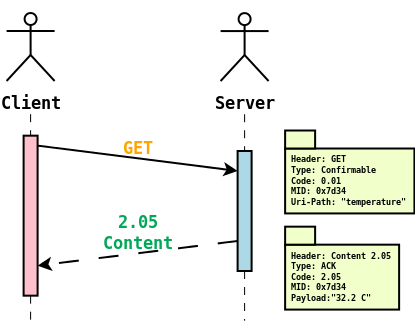
\includegraphics[width=0.6\textwidth]{figuras/piggybacked.png}
   \caption{Resposta na mensagem de confirma\c{c}\~ao, chamado de piggy-backed.}
\end{figure}

Fluxo esperado de requisi\c{c}\~ao sem confirma\c{c}\~ao na figura \ref{nonConfirmable}.
\begin{figure}[h]
   \label{nonConfirmable}
   \centering
   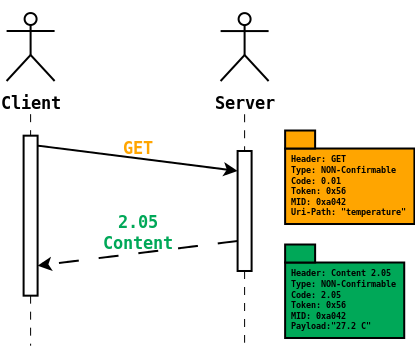
\includegraphics[width=0.6\textwidth]{figuras/nonconfirmable.png}
   \caption{Fluxo esperado de requisi\c{c}\~ao e resposta sem confirma\c{c}\~ao}
\end{figure}

A RFC tamb\'em prev\^e fluxo de requisi\c{c}\~ao com confirma\c{c}\~ao, e resposta separada com confirma\c{c}\~ao. A figura \ref{separateResponse} exemplifica:

\begin{figure}[h]
   \label{separateResponse}
   \centering
   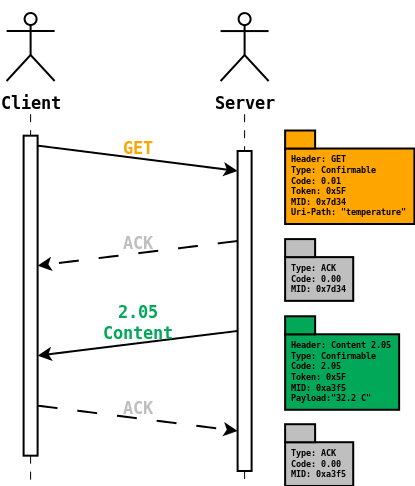
\includegraphics[width=0.6\textwidth]{figuras/separateresponse.png}
   \caption{Fluxo esperado de requisi\c{c}\~ao e resposta com confirma\c{c}\~ao, com resposta separada}
\end{figure}

\subsection{Camada de Reposta e Requisi\c{c}\~ao}
Uma requisi\c{c}\~ao \'e inicializada ao preencher o campo code no cabe\c{c}alho do CoAP. Possuem as mesmas propriedades de idempot\'encia e only retrieved das requisi\c{c}\~oes HTTP.

\subsection{Recursos}
A descoberta de recursos \'e feita quando um servidor recebe uma requisi\c{c}\~ao GET para o recurso ~/well-know/core. O servidor CoAP deve responder no formato CORE link Format.\cite{rfc6690} E a descoberta de servi\c{c}os no protocolo CoAP \'e feita atrav\'es de socket Multicast. Os recursos s\~ao identificados por uma URI, e os m\'etodos s\~ao implementados de forma similar ao HTTP.

\afazer{A desenvolver...}

%Inserir figura que represente os recursos ???

\section{EPOS}
O EPOS \'e um sistema operacional multithread com suporte a preemp\c{c}\~ao, foi desenvolvido em C++ que faz uso intenso de programa\c{c}\~ao orientada a aspectos utilizando templates.

Possui abstra\c{c}\~oes para entidades temporais como rel\'ogio, alarme e cron\^ometro, biblioteca com estruturas de dados e sequenciadores. Permitindo o uso de ferramentas para gera\c{c}\~ao automatizada de abstra\c{c}\~oes de sistemas. A portabilidade \'e atingida utilizando entidades chamados de Mediadores de Hardware que fornecem interfaces simples para acesso as fun\c{c}\~oes espec\'ificas de arquitetura. Estas interfaces s\~ao utilizadas por entidades abstratas como alarmes e threads peri\'odicas. A figura 5 mostra uma vis\~ao abstrata da arquitetura do EPOS.

%Inserir figura da arquitetura do EPOS.

Foi projetado utilizando ADESD, Application Driven Embedded System Design, um m\'etodo para projeto de sistemas embarcados orientados \`a aplica\c{c}\~ao. Esta metodologia guia o desenvolvimento paralelo de hardware e software al\'em de manter portabilidade. O EPOS possui porte para as seguintes arquiteturas: MIPS, IA32, PowerPC, H8, Sparc, AVR e ARM. \cite{epos}

Utiliza um sistema de constru\c{c}\~ao baseado em makefiles e shell scripts.

\section{Trabalhos Relacionados}

\subsection{OpenMote}

\subsection{OpenWSN}

O projeto OpenWSN \'e um projeto de visa o c\'odigo aberto e confia na comunidade para manter atualizado e encontrar erros. Possui uma implementa\c{c}\~ao completa de c\'odigo aberto, das pilhas de protocolos padr\~oes pra Internet das Coisas. E com a primeira implementa\c{c}\~ao aberta do padr\~ao 802.15.4e, Time Synchronized Channel Hopping.

Por serem sincronizados os motes precisam acordar apenas para transmitir ou receber e periodicamente se comunicar para manter a rede sincronizada quando estiver inativo. Este overhead de temporiza\c{c}\~ao \'e pequeno, cerca de 0.02\% de ciclo de trabalho do r\'adio. \cite{openWSNPaper}

O pilha de protocolos \'e totalmente em C e pode ser compilada em qualquer toolchain que suporte uma plataforma alvo. OpenWSN j\'a foi portado para as seguintes arquiteturas: ARM, AVR, ...

Possui porte para diversas plataformas de microcontroladores de 16 bits e para as arquiteturas mais novas de 32 bits dos cortex-M. O projeto possui diversas ferramentas para depura\c{c}\~ao, simula\c{c}\~ao e ambiente necess\'ario para integrar as aplica\c{c}\~oes a Internet.\cite{openWSN}

Resultados experimentais de uma rede de motes demonstram que os r\'adios operam num ciclo m\'edio de trabalho de $0.1\%$ e uma m\'edia de 0.68 microA em hardware comum. Este consumo baixo permite uma vasta gama de aplica\c{c}\~oes.

Para utilizar \'e necess\'ario baixar os seguintes reposit\'orios:
\begin{itemize}
    \item Software de sistema que ir\'a executar no simulador ou nos motes:\\https://github.com/openwsn-berkeley/openwsn-fw
    \item Ferramentas que ir\~ao executar no computador de desenvolvimento:\\https://github.com/openwsn-berkeley/openwsn-sw 
    \item Implementa\c{c}\~ao do CoAP em Python:\\https://github.com/openwsn-berkeley/coap
\end{itemize}


\subsection{Contiki}
O Contiki \'e um sistema operacional criado por Adam Dunkels em 2000, escrito em C, de c\'odigo aberto para sistemas com restri\c{c}\~ao de recursos comunicam-se numa rede. Foi desenvolvido para ser um sistema operacional para Internet das coisas. Possui uma camada de abstra\c{c}\~ao RESTful para web services chamada Erbium, que implementa o protocolo CoAP.

Cada processo no Contiki possui bloco de controle, que cont\'em informa\-\c{c}\~oes de tempo de execu\c{c}\~ao do processo e uma refer\^encia para uma protothread, na qual o c\'ogido \'e armazenado na ROM. 

Protothread \'e uma combina\c{c}\~ao entre eventos e threads, possuem comportamentos de bloqueio e espera, que permite o intersequenciamento dos eventos, gerando um baixo overhead de mem\'oria por n\~ao necessitar de salvamento de contexto.

Cada protothread consome 2 bytes de mem\'oria, que s\~ao utilizados para armazenar a continuidade local, uma referencia utilizada em um pulo condicional durante a execu\c{c}\~ao da thread. \'E um m\'etodo similar ao mecanismo de Duffy e Co-rotina em C. \cite{duffy}

O transceiver sem fio \'e um dos componentes que mais consome energia quando ligado escutando o ambiente, assim uma das estrat\'egias utilizadas \'e manter o m\'inimo de tempo poss\'ivel ligado, mas o suficiente para manter a troca de mensagens na rede. O Contiki prop\~oe uma estrat\'egia de ciclos de trabalho que consegue manter um n\'o comunic\'avel em uma rede, por\'em com seus r\'adios desligados em aproximadamente 99\% do tempo.

\subsection{LibCoap}
LibCoap \'e uma biblioteca implementada em C do protocolo CoAP. Possui 292K de tamanho compilada estaticamente em sua vers\~ao 4.0.1.
A licensa da biblioteca \'e GPL (2 ou maior) ou licensa BSD revisada.

Possui uma su\'ite de testes para regress\~ao, utilizando o framework de testes CUnit (http://cunit.sourceforge.net/). A documenta\c{c}\~ao pode ser encontrada em: http://libcoap.sourceforge.net/.

\'E uma biblioteca auto-condida, que possui parser do protocolo e fun\c{c}\~oes b\'asicas de rede utilizando sockets tipo BSD e malloc. Implementa\c{c}\~ao de Hash, String e URI: os headers s\~ao hashkey.h, str.h, uri.h utilizados para montar os pacotes CoAP.

\'E separada num m\'odulo de rede: net.h, aonde \'e implementado as fun\c{c}\~oes de envio/recebimento de requisi\c{c}\~oes e respostas, com confirma\c{c}\~ao, sem confirma\c\~ao, mensagem de reset e erros.

Para selecionar a camada de transporte \'e necess\'ario selecionar utilizando flags de preprocessamento. O padr\~ao \'e socket POSIX. A pilha uIP \'e selecionada com a flag -DWITH\textunderscore CONTIKI, ou para selecionar a pilha lwIP -DWITH\textunderscore LWIP.

\subsection{TinyOS}
O TinyOS \'e um sistema operacional projetado para sistemas embarcados com comunica\c{c}\~ao sem fio e restri\c{c}\~oes energ\'eticas. Foi desenvolvido em nesC, uma linguagem c\'odigo aberto que \'e uma extens\~ao do C. \'E um sistema operacional baseado em eventos desenvolvido para redes de sensores que possuem recursos limitados. Possui uma implementa\c{c}\~ao do CoAP baseada na libCoAP.

\subsection{CantCoap}
\'E uma implementa\c{c}\~ao em C++ que visa facilitar a cria\c{c}\~ao de pacotes Coap tanto diretamente quanto a partir de uma sequ\^encia de characteres, recebida da camada UDP por exemplo.

\'E poss\'ivel montar os pacotes CoAP a partir de uma sequ\^encia de caracteres recebidos de uma placa de rede. Abaixo exemplos de uso da biblioteca retirados de https://github.com/staropram/cantcoap.

\lstdefinestyle{customc}{
  belowcaptionskip=1\baselineskip,
  breaklines=true,
  xleftmargin=\parindent,
  language=C++,
  showstringspaces=false,
  basicstyle=\scriptsize\ttfamily,
  keywordstyle=\bfseries\color{green!40!black},
  commentstyle=\itshape\color{blue},
  identifierstyle=\color{blue!20!black},
  stringstyle=\color{red},
}

\lstset{escapechar=@,style=customc}

Abaixo um exemplo de uso para montar um pacote e enviar:

\begin{lstlisting}
CoapPDU *pdu = new CoapPDU();
pdu->setType(CoapPDU::COAP_CONFIRMABLE);
pdu->setCode(CoapPDU::COAP_GET);
pdu->setToken((uint8_t*)"\3\2\1\0",4);
pdu->setMessageID(0x0005);
pdu->setURI((char*)"test",4);

// send packet 
ret = send(sockfd,pdu->getPDUPointer(),pdu->getPDULength(),0);
\end{lstlisting}

Quando receber a mensagem a forma de uso \'e mostrada abaixo:
\begin{lstlisting}
// receive packet
ret = recvfrom(sockfd,&buffer,BUF_LEN,0,recvAddr,recvAddrLen);
CoapPDU *recvPDU = new CoapPDU((uint8_t*)buffer,ret);
if(recvPDU->validate()) {
    recvPDU->getURI(uriBuffer,URI_BUF_LEN,&recvURILen);
    ...
}
\end{lstlisting}

Por ser uma biblioteca bem simplificada e n\~ao possuir depend\^encias diretas com a implementa\c{c}\~ao da camada de transporte e ser c\'odigo livre, foi escolhida para a implementa\c{c}\~ao teste do trabalho.
